\chapter{Discussions}\label{chap:discussions}
\begin{chapabstract}

In this Chapter, we show further discussion on our results in Chapter~\ref{chap:results}.
Section~\ref{sec:comparingthecalibration} compares our fitting results, mainly the frequency dependence of $\qn$ with previous studies.
Section~\ref{sec:radiosfruncertainty} shows the comparison of the radio SFR calibration with \citet{CalistroRivera2017a}.
Section~\ref{sec:galaxypropertiesfortheradiosfr} describes how galaxy properties affect the SFR estimation.
Here, we focus on the active galactic nuclei in a galaxy and the \nh-deficiency.
Section~\ref{sec:nondetectedgalaxiesbythegleamsurvey} describes HRS galaxies whose radio counterparts are not detected by the GLEAM survey.
In this Section, we also mention the possibility of their radio source detection by the updated GLEAM survey.

\end{chapabstract}

\section{Comparing the Calibration with Previous Results}\label{sec:comparingthecalibration}

Here, we compare our results in Section~\ref{sec:GammaDistribution} with previous research.
From our samples, we obtain the mean $\gamma=-0.63 \pm 0.07$ from the fitting between MWA frequencies and $1500\MHz$.
\citet{CalistroRivera2017a} and \citet{Chyzy2018} obtained $-0.78 \pm 0.24$ and $-0.56 \pm 0.11$, respectively.

\begin{figure}[htbp]
	\centering
	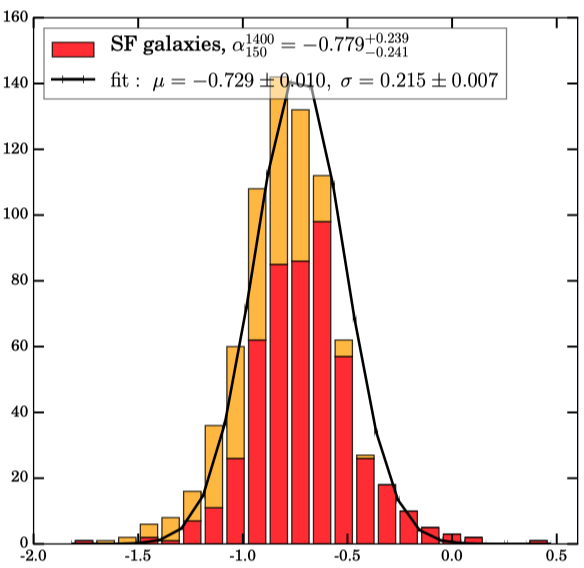
\includegraphics[width=.7\linewidth]{Chapter_6/Figures/CalistroRivera2017_Figure7.png}
    \caption[The histogram of the spectral index in \citet{CalistroRivera2017a}]{\label{fig:CalistroRivera2017_figure7}
        The histogram of the spectral index corresponding to $\gamma$ in this study.
        They calculate it between $150\MHz$ (LOFAR;~\citealt{Williams2016}) and $1.4\GHz$ (Westerbork Synthesis Radio Telescope, WSRT;~\citealt{DeVries2002}).
        Red and orange histograms show the samples detected and non-detected by WSRT\@.
        To estimate the flux of non-detected samples, they extract aperture fluxes from the source location known by LOFAR on the radio map (forced photometry technique).
        The black solid line displays the Gaussian fitting function.
        They put the average $\mu$ and standard deviation $\sigma$ from the fitting on the upper right in the figure.
        Adapted from \citealt{CalistroRivera2017a}, Figure~7.
    }
\end{figure}

\begin{figure}[htbp]
	\centering
	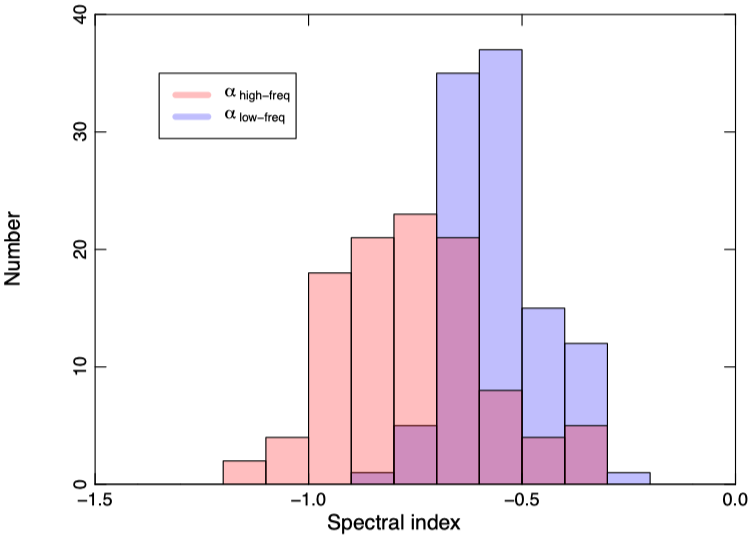
\includegraphics[width=.8\linewidth]{Chapter_6/Figures/Chyzy2018_Figure4.png}
    \caption[The histogram of the spectral index in \citet{Chyzy2018}]{\label{fig:Chyzy2018_figure4}
        Red and blue histograms show the spectral index corresponding to $\gamma$ in this study calculated fluxes from $1.3\GHz$ to $5\GHz$ and $150\MHz$ to $1.4\GHz$, respectively.
        They show histogram in violet where they are overlapping.
        From the definition, we should compare our result with the blue one.
        They calculate it between $150\MHz$ (The Multifrequency Snapshot Sky Survey, MSSS;~\citealt{Heald2015}) and $1.4\GHz$ (the NRAO VLA Sky Survey, NVSS;~\citealt{Condon1998}).
        Adapted from \citealt{Chyzy2018}, Figure~4.
    }
\end{figure}

The difference of these might result from the selection of galaxy samples.
While we use nearby galaxies within $25\,\mr{Mpc}$, \citet{CalistroRivera2017a} do 758 galaxies up to $z\sim2$, and \citet{Chyzy2018} do 118 galaxies up to $z=0.04$.

\citet{Chyzy2018} indicate that the slope is steeper at higher frequencies ($1.3 \sim 5\GHz$), and this might steepen the slope of galaxy samples in \citet{CalistroRivera2017a} which adopt galaxies up to $z\sim2$.
Since \citet{CalistroRivera2017a} did not execute $k$-correction for Figure~\ref{fig:CalistroRivera2017_figure7}, some $\alpha$ values indicate the spectral index at higher frequencies, which might be expected to have a steeper slope.
Considering the value and scatter, our result using the Herschel reference sample would be consistent with previous findings.
Indeed, the frequency dependence of the low-frequency emission and its relation with IR emission is still uncertain.



\section{Uncertainty of Radio SFR}\label{sec:radiosfruncertainty}

In Section~\ref{sec:sfrfromlowradio}, we show the consistency of our SFR calibrations using the low-frequency emission.
For calculating the more accurate radio SFR, we need its spectral energy distribution for each galaxy, as we have already shown in Section~\ref{sec:sfrfromlowradio}.
Since star-forming galaxies have a wide variety of $\qn$ at low frequencies ($\sim 0.53\,\mr{dex}$ in Figure~14, 15; \citealt{CalistroRivera2017a}) and still we do not know the physical details, the radio SFR calibration has considerable uncertainty.
Substituting averaged $\gamma$ and $\q{1500\MHz}$ obtained from our sample galaxies into Equation~\ref{eq:sfrfromradio} yields the following equation:

\begin{equation}\label{eq:sfrradio_calibration}
    \mr{SFR}_{\mr{Radio},\,150\MHz} = \brp{1.03\pm0.27} \times 10^{-29} \times \brp{\frac{L_{\mr{Radio},\,150\MHz}}{\brb{\mr{erg}\,\mr{s}^{-1}}}}
\end{equation}
where we substitute the median values of $\gamma=-0.63$, $\q{1500\MHz}=2.48$ from our samples and $\nu=150\MHz$ into Equation~\ref{eq:sfrfromradio}.

\citet{CalistroRivera2017a} have obtained the coefficient of $0.76 \pm 0.08$ in Equation~\ref{eq:sfrradio_calibration} for nearby galaxies ($z = 0$) from their calibration.

We should keep our mind that the SFR calibration has non-negligible uncertainty, possibly caused by the galaxy selection and the variety of $\qn$ at low frequencies.
For estimating SFR accurately, we need the radio spectral with multi-band observation.



\section{Galaxy Properties for the Radio SFR}\label{sec:galaxypropertiesfortheradiosfr}

In this Section, we discuss how the galaxy property affect the results mentioned in previous Sections.
Here, we focus on the central engine and the environment of a galaxy.
The central engine in a galaxy driven by the supermassive black hole and the baryon accretion is called active galactic nuclei and known as another radio source.
Although we have eliminated galaxies which have strong radio emission against their star formation activity in Section~\ref{sec:reducegalaxysamples}, there are still some galaxies in our sample, which might have an active galactic nuclei identified by the optical line emissions.
%These kinds of galaxies that might have a strong radio emission are called Seyfert or LINER galaxies.
They might be related to Seyfert or LINER galaxies. 
And they possibly affect our results due to their radio emissions irrelevant to the star-formation activity.
Here, we investigate this property using the BPT diagram mentioned in Section~\ref{sec:GammaDistribution} and find three galaxies (HRS 144, 163 and 220) in our sample that have sharp optical emission lines (Figure~\ref{fig:bpt_diagram}).
In the BPT diagram, HRS 144 and 163 are found to be Seyfert galaxies, and HRS 220 is LINER galaxy.

\begin{figure}[htbp]
	\centering
	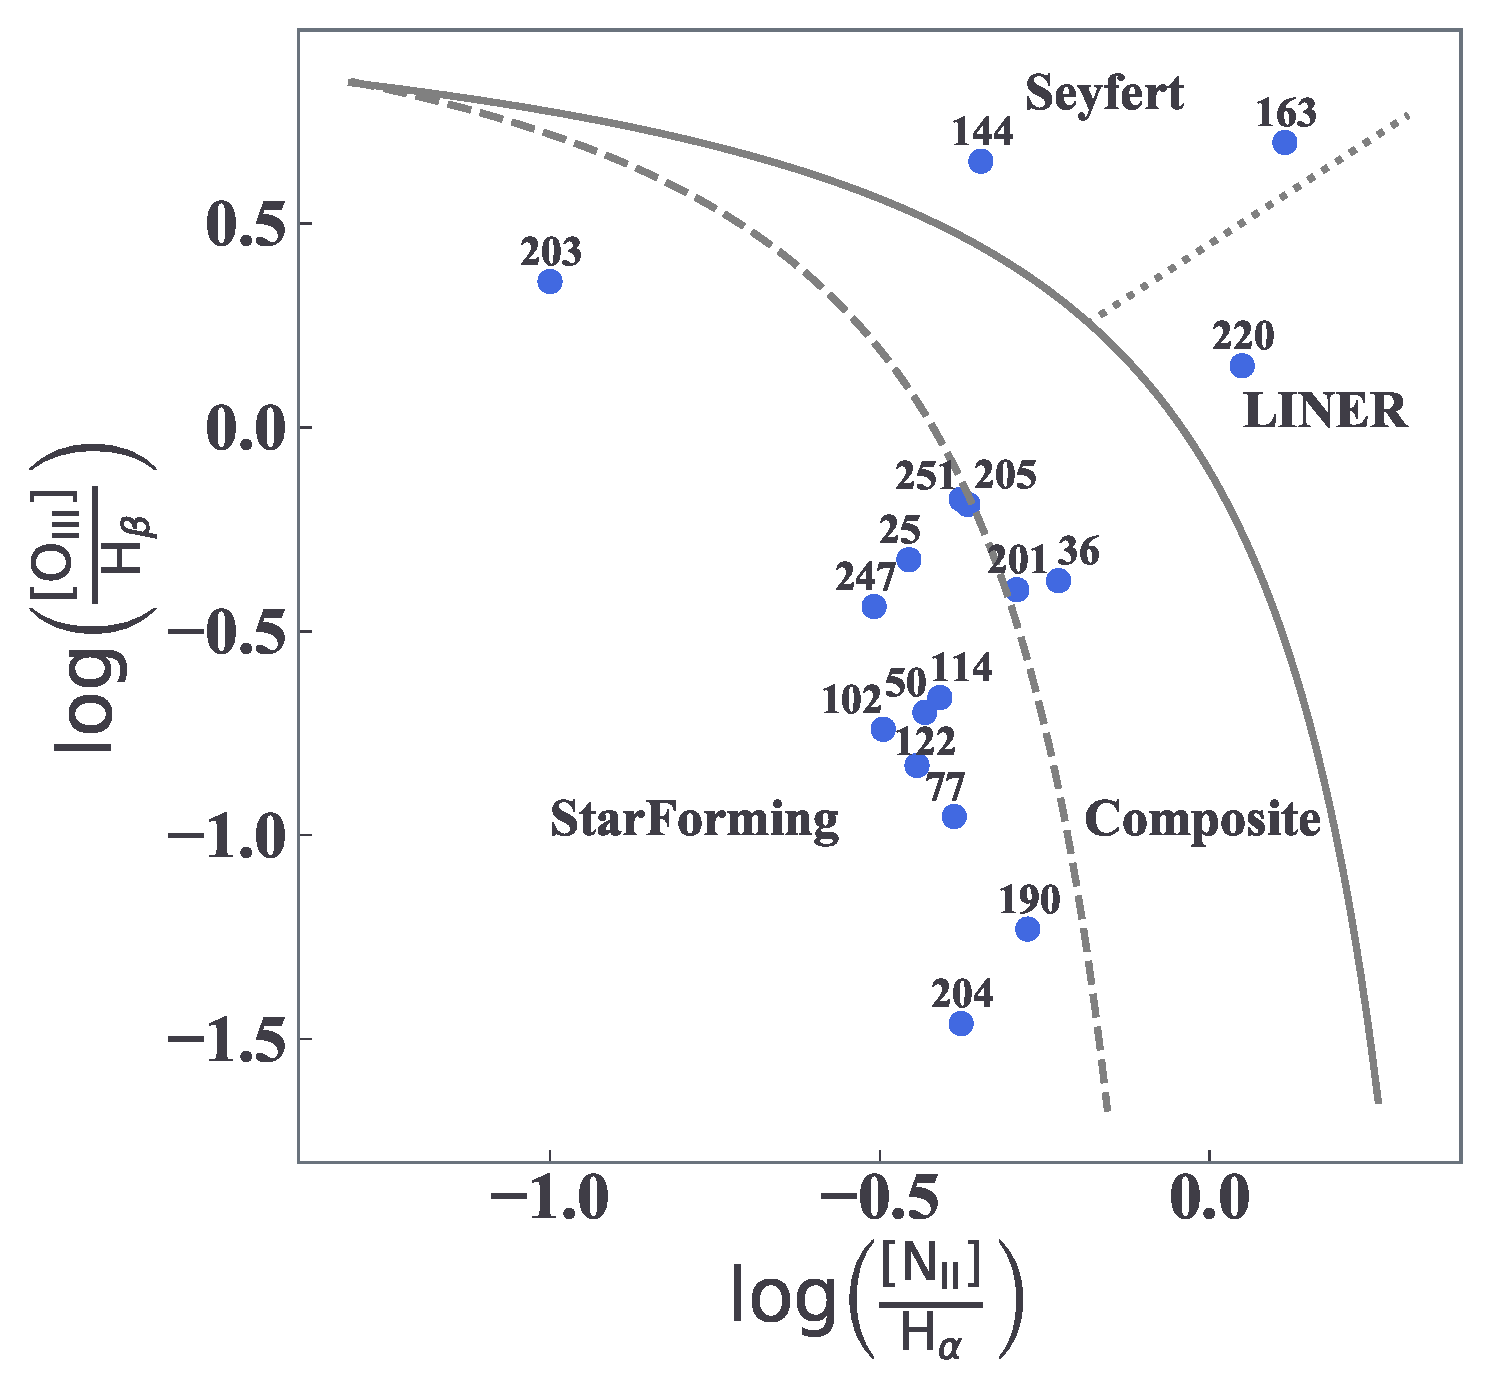
\includegraphics[width=.8\linewidth]{Chapter_6/Figures/Discuss_bpt.pdf}
    \caption[BPT diagram for 18 galaxy samples]{\label{fig:bpt_diagram}
        The BPT diagram is for 18 galaxy samples.
        Since HRS 306 does not have any line emission data, we do not plot it on the plot.
        The solid, dashed and dotted lines show the borders of different kinds of nuclei.
        We draw these lines based on \citet{Kewley2001}, \citet{Kauffmann2003} and \citet{Schawinski2007}, respectively.
    }
\end{figure}

After that, we also examine the galaxy environment of each galaxy.
\citet{Boselli2014} have already calculated the \nh-deficiency (\nh-def) for all HRS galaxies.
\nh-deficient galaxy is defined as a galaxy whose the \nh~mass is much smaller than the expected one based on the morphology and the size of a galaxy \citep{Haynes1984, Boselli2009}.

The definition of \nh-deficiency is as follows:

\begin{equation}\label{eq:definitionofHIdeficiency}
    \text{\nh-def} = \log\brp{M\msb{\nh,\,expected}} - \log\brp{M\msb{\nh,\,observed}}
\end{equation}
where $\log\brp{M\msb{\nh,\,expected}}$ is defined by \citet{Haynes1984}:

\begin{equation}\label{eq:definitionofexpectedHIdef}
    \log\brp{h^2 M\msb{\nh,\,expected}} = c + d\log\brp{h\times\mr{diam}}^2
\end{equation}
where $c$ and $d$ are weak functions of the galaxy morphology, $\mr{diam}$ is the linear diameter of the galaxy and $h=H_0 / 100$.

Here, we regard a galaxy whose \nh-deficiency is more than 0.4 as a \nh-deficient galaxy and the other case as a normal galaxy, which is the same criteria in \citet{Ciesla2016}.
\nh-deficiency is known to represent not only the amount of the \nh~mass but also a galaxy environment.
This is because \nh-deficiency might be attributed to the tidal stripping or ram pressure, which happens in the dense region (e.g., the center of a cluster).
Therefore, we can roughly assume that \nh-deficient galaxies are located in the dense regions, and normal galaxies are the field galaxies.
The relation between a galaxy environment and low-frequency emissions are still not fully understood.
However, there is a possible scenario to distort the magnetic field and strengthen the synchrotron radiation due to the frozen-in of the magnetic field with the stripped \nh~gas \citep{Murphy2009}.

Firstly, we show the result of a spectral index distribution (Figure~\ref{fig:comparehist}) with the labeling.
In Figure~\ref{fig:comparehist_h1def}, we cannot see the significant difference between normal galaxies and the others in the left figure.
But in the right one, we can see the \nh-deficient galaxies tend to have a scattered spectral index.
This suggests that the galaxy environment might affect the energy distribution of high-energy electrons, which directly related to the spectral index.
%Unfortunately, in our sample, we do not find the significant difference for Seyfert or LINER galaxies, but cannot reject the possibility that these AGNs vary the spectral index.
For Seyfert and LINER galaxies, we can see relatively steep $\gamma$ in the histogram.
However, we cannot conclude it is intrinsic effect from AGNs because of the small sample size and indistinguishable properties (\nh-deficient and AGNs).

\begin{figure}[htbp]
	\centering
	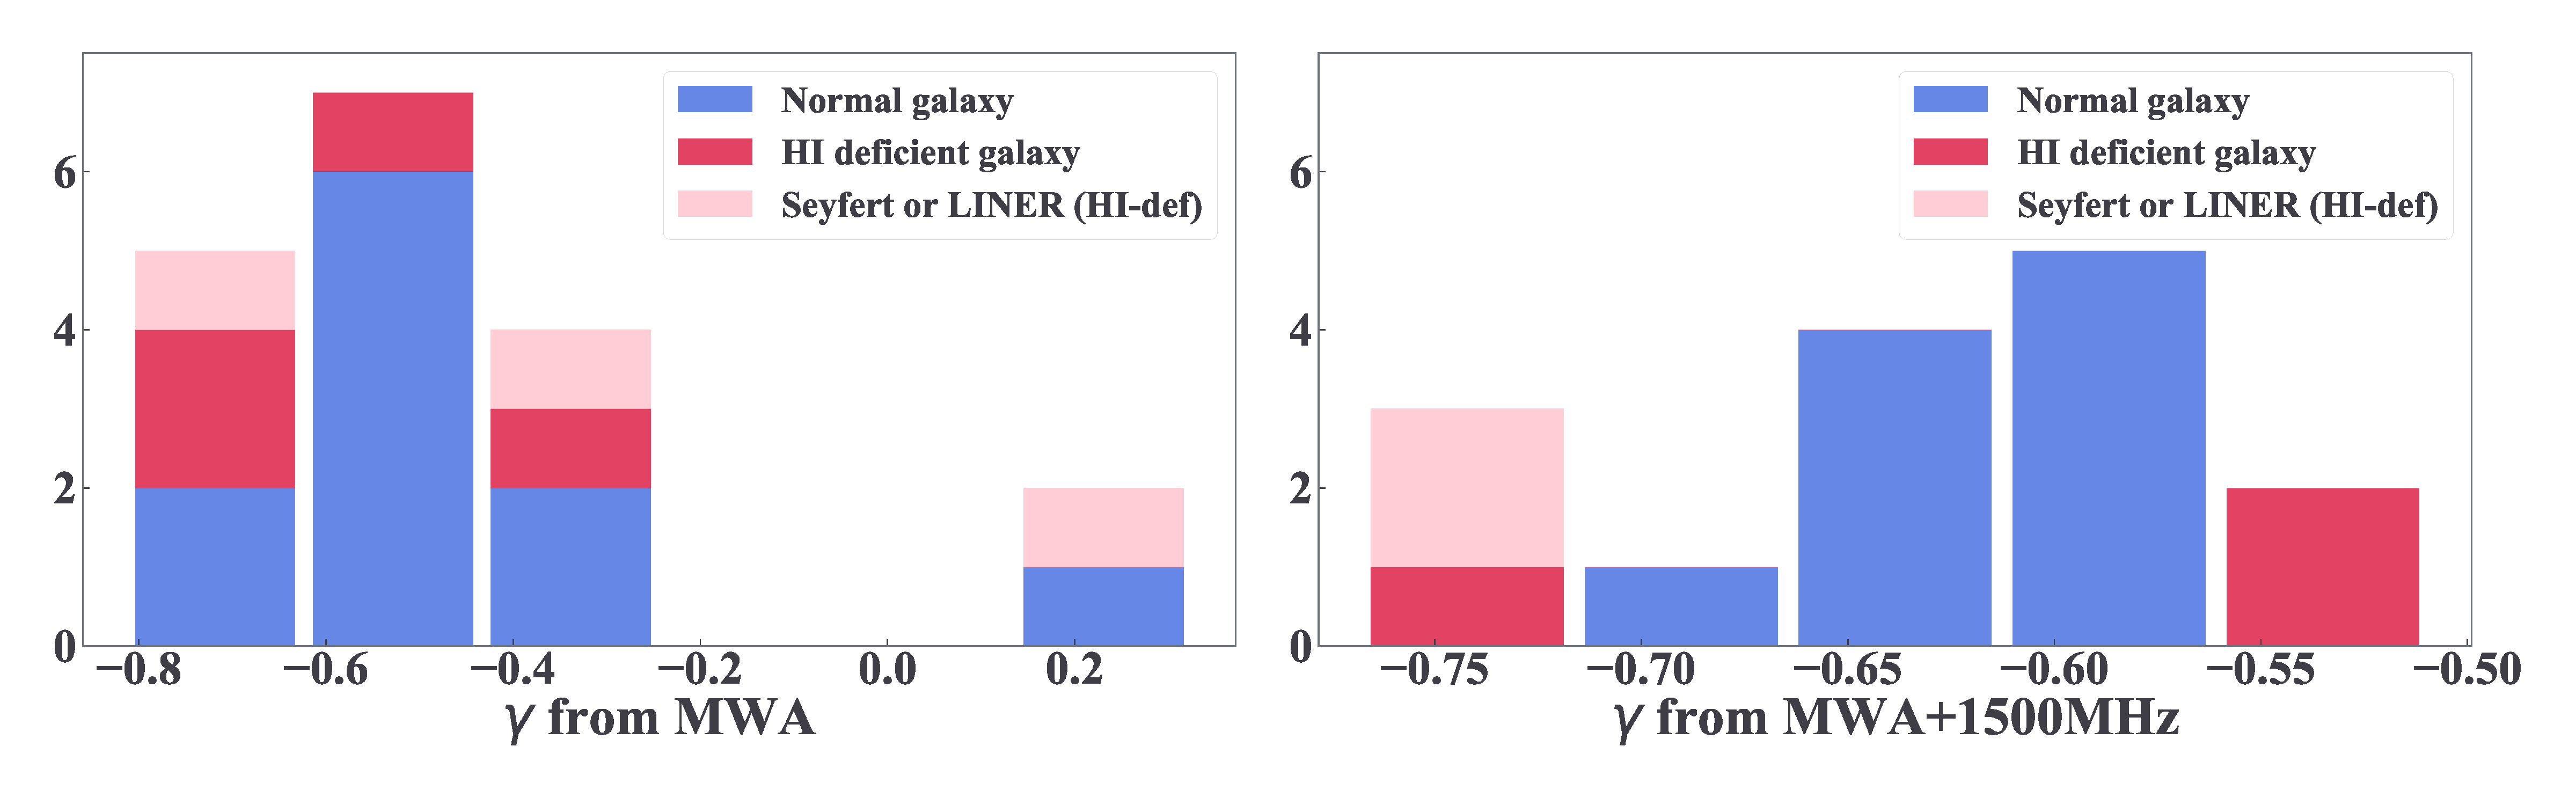
\includegraphics[width=\linewidth]{Chapter_6/Figures/Discuss_comparehist.pdf}
    \caption[Histograms of $\gamma$ from the fitting (labeled)]{\label{fig:comparehist_h1def}
        The spectral index distribution obtained from the two kinds of fitting as same as in Figure~\ref{fig:comparehist}.
        Here, we make a histogram with color labeling based on the galaxy properties mentioned in Section~\ref{sec:galaxypropertiesfortheradiosfr}.
        The blue histogram shows the normal galaxies; red one shows the HI deficient galaxies (\nh-def $> 0.4$), and the pink shows the Seyfert or LINER galaxies with \nh-deficient.
        Our sample does not have the galaxy, which is Seyfert or LINER without \nh-deficient.
        Although the left figure does not show the significant difference between normal galaxies and the others, the right figure shows the \nh~deficient galaxies tend to have a scatter spectral index compared to the normal galaxies.
    }
\end{figure}


Secondly, we show the $\qn$ value plots with the label of galaxy properties mentioned above.
This $\qn$ value plot helps us to understand how the galaxy property affects the SFR ratio in Figure~\ref{fig:sfrratio}.
As we have mentioned in Section~\ref{sec:sfrfromlowradio}, the $\qn$ value variation makes a larger scatter of SFR ratio when we estimate $\mr{SFR}_{\mr{Radio},\,\nu}$ with averaged parameters.

\begin{figure}[htbp]
	\centering
	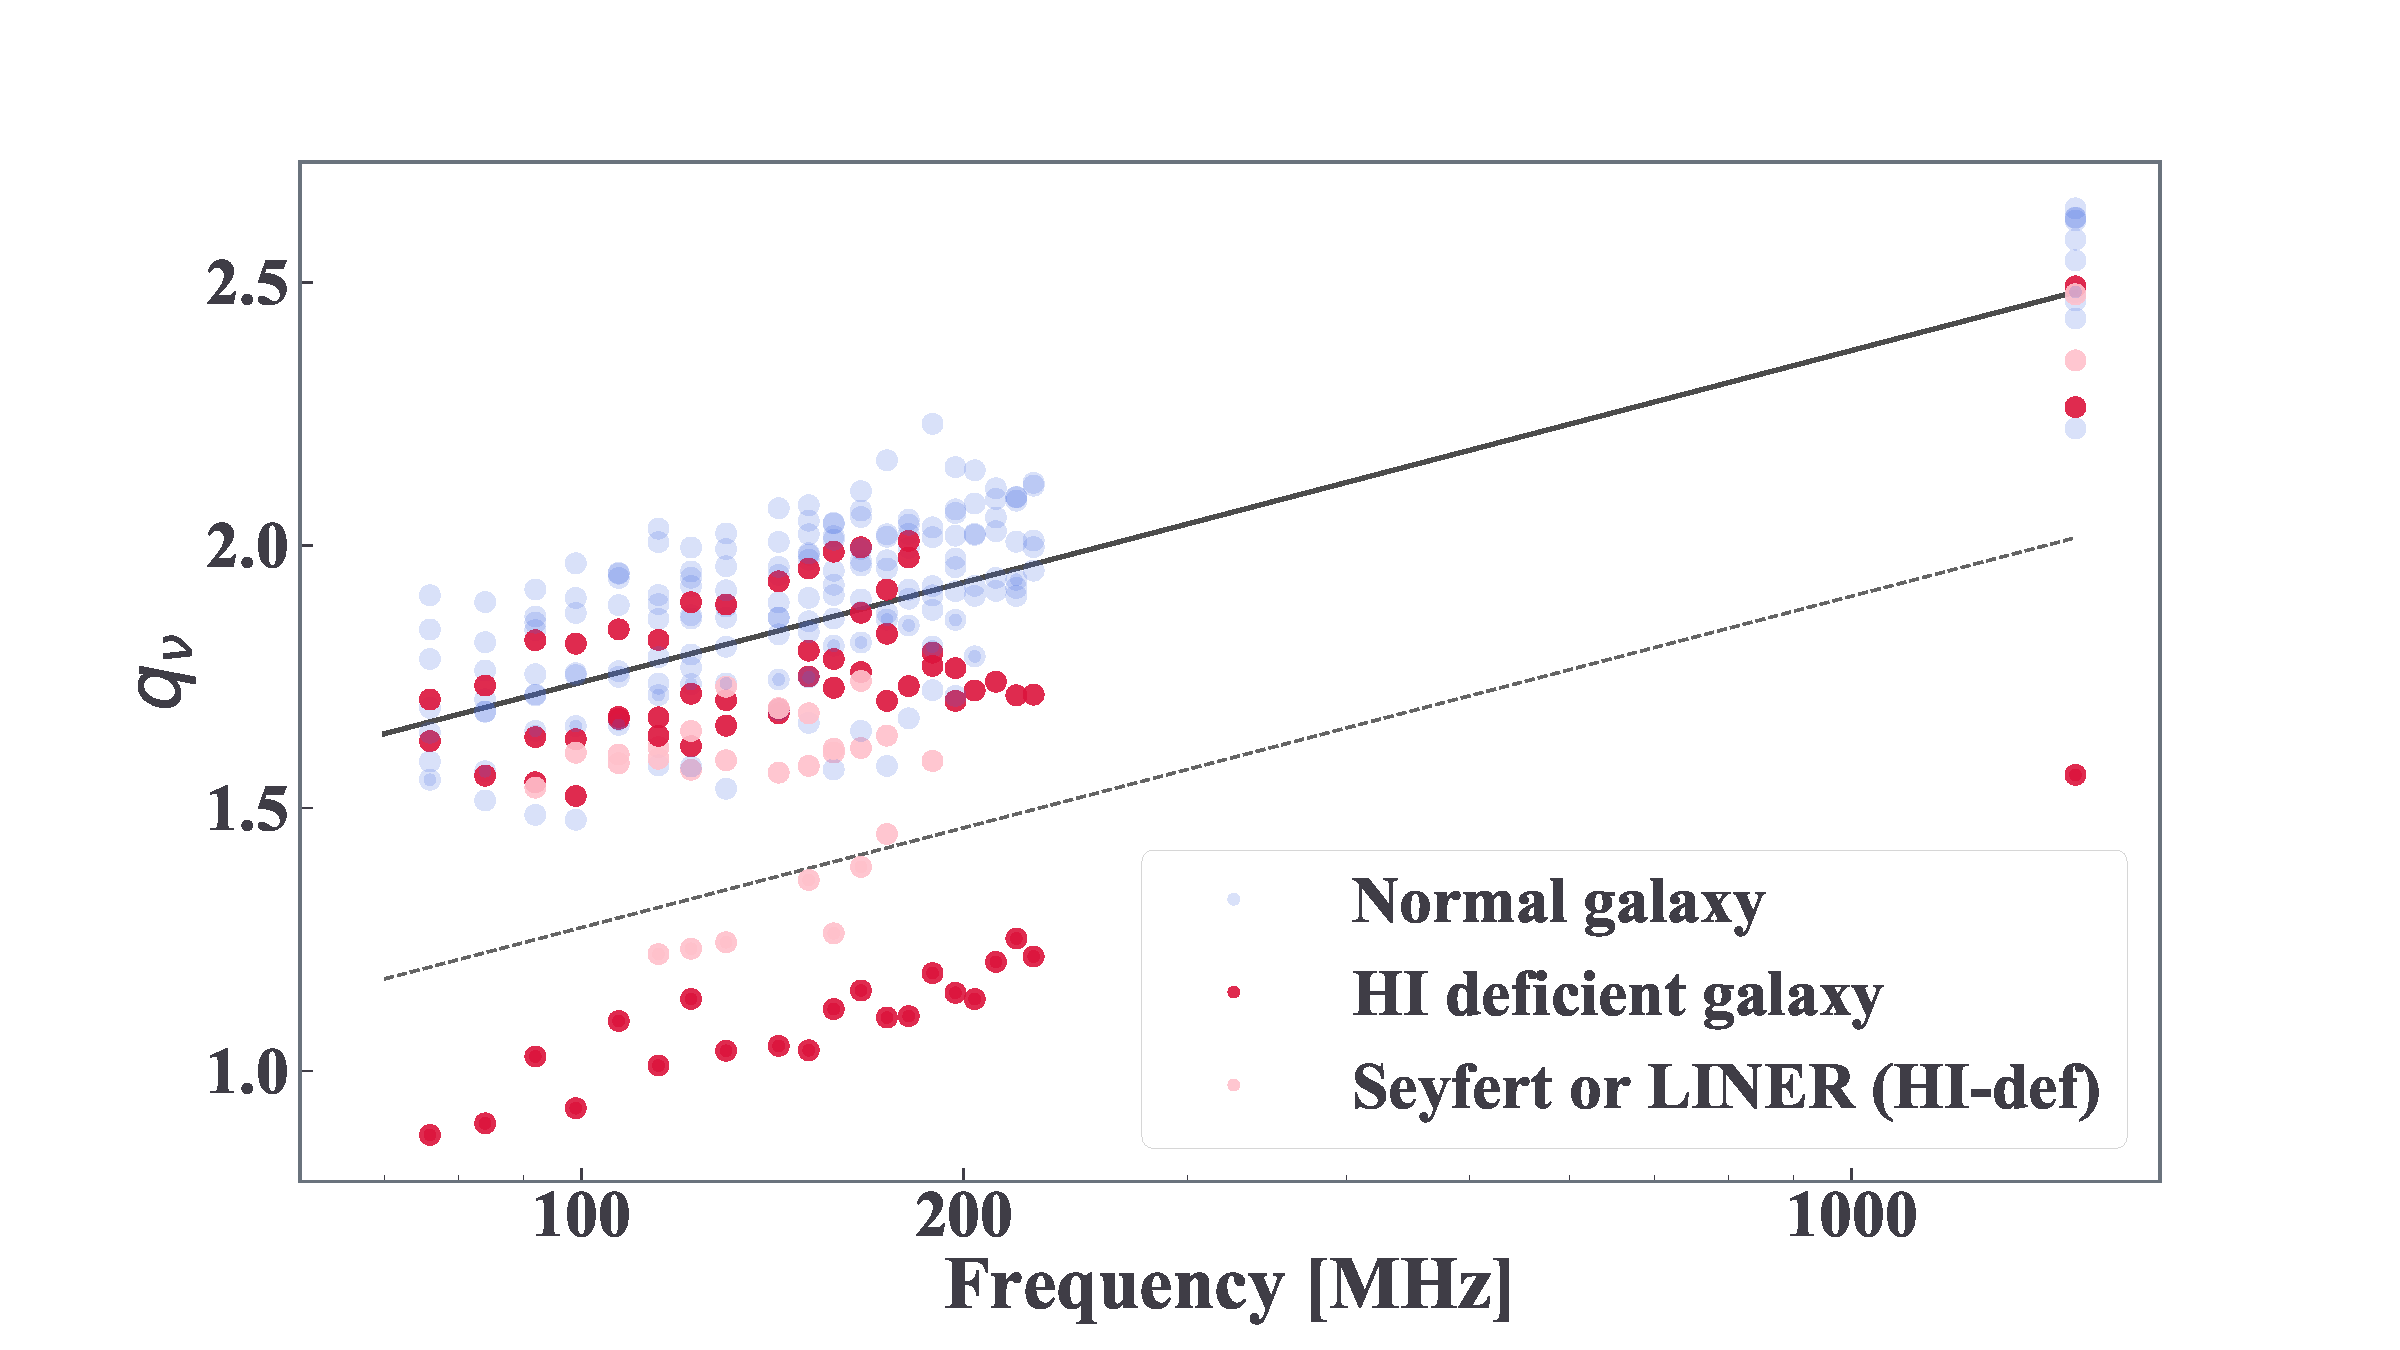
\includegraphics[width=\linewidth]{Chapter_6/Figures/Discuss_compareq.pdf}
    \caption[$\qn$ plots for each galaxy with labels]{\label{fig:comparehist_q}
        The $q_{\nu}$ value distribution at MWA frequencies and $1500\MHz$.
        The solid black line is the extrapolate line from the median value of $\q{1500\MHz}$ to the MWA frequencies with the median spectral index $\gamma$.
        For calculating $\mr{SFR}_{\mr{Radio},\,\nu}$, we have used this extrapolation. The dotted black line is the border for showing the outliers below this line.
        The plots below this line arise from only two galaxies, and we can say these are the outliers.
        In this figure, we can see the most plots distributing around the solid black line, which shows the extrapolated median value from $\q{1500\MHz}$.
        But we also find there are two galaxies (HRS 163 and 306) that have lower values in a whole frequency range.
    }
\end{figure}

In Figure~\ref{fig:comparehist_q}, we can see some \nh-deficient galaxies and Seyfert or LINER galaxies tend to have smaller $\qn$ values, which means they have stronger radio emissions.
As I have already mentioned, \nh-deficient galaxies would have amplified synchrotron radiation caused by the distortion of their magnetic field.
Figure~\ref{fig:comparehist_q} shows that \nh-deficient galaxies including AGNs have relatively smaller $\qn$ (stronger radio emission), and this result might support the scenario.
We also find that there are two galaxies (HRS 163 and 306), which have significantly lower $\qn$ values.
Since galaxies which have stronger radio emissions might possess the other radio source rather than the star formation activity in addition to the effect of the magnetic distortion, we should not estimate SFR from radio emissions for these galaxies.
Indeed, these two galaxies are outliers on the right plot in Figure~\ref{fig:sfrratios} and apparently these make non-negligible uncertainty.

For the reliable SFR estimation with the low-frequency emission, we definitely need to classify which galaxies are appropriate for calculating their SFR from radio emissions.
However, due to our sample size, we cannot conclude how much $\qn$ value is safe for executing the SFR estimation from the low-frequency emission.
In future studies, we should clarify the distribution of this plot and find borders of $\qn$ for reliable SFR estimation.


\section{Non-detected Galaxies by the GLEAM Survey}\label{sec:nondetectedgalaxiesbythegleamsurvey}

Here, we mention galaxies that have not been observed by the GLEAM survey.
In this study, we have found 39 HRS galaxies have a potential radio counterpart in the GLEAM survey in Section~\ref{sec:crossmatching}.
So in this Section, we focus on other 283 HRS galaxies.

Firstly, we check the coordinate of these galaxies, and peeled sources which was removed during the data reduction for compiling the GLEAM catalog.
Out of 283 galaxies, we confirm 44 galaxies are out of the observational region by the GLEAM survey, and HRS 183 (M87, Virgo A) is peeled because of its too strong radio emission.
\citet{Hurley-Walker2017a} peeled radio sources expected to be more than $50\,\mr{Jy}$ in apparent flux density from the visibilities for reducing the grating sidelobes.
So we confirm these 45 galaxies have reasonable reasons why their radio sources are not on the GLEAM catalog.
However, the other 238 out of 283 galaxies do not have understandable reasons.

Secondly, we examine the flux values at $200\MHz$ because their non-detection is reasonable if the expected flux value is lower than the detection limit.
In this analysis, we extrapolate the flux at $200\MHz$ from $1500\MHz$ \citep{Boselli2015} with $S \propto \nu^{\gamma}$ $\brp{\gamma = -0.63\ \text{obtained in this study}}$ and compare it with the rms noise described in \citet{Hurley-Walker2017a}.
Note that the rms noise is different depends on the declination, so we apply $\sigma\msb{rms} = 10$ for galaxies at $-72^{\circ} \leq \mr{Dec} \leq 18^{\circ}.5$ and $\sigma\msb{rms} = 28$ for galaxies at $18^{\circ}.5 \leq \mr{Dec}$.
Also, we should mention that we can analyze only 107 galaxies because other the 131 galaxies do not have a high-quality flux data at $1500\MHz$ \citep{Boselli2015}.
After all, we find 34 galaxies have extrapolated flux at $200\MHz$ higher than $5\sigma\msb{rms}$.
This result means that these 34 galaxies should have been observed by the GLEAM survey, but they were not.
One possible reason for the non-detection of these galaxies is a flatter radio spectral.
Here, we assume $\gamma = -0.63$ for the extrapolation.
However, if these galaxies have a flatter spectral, the flux of these galaxies at $200\MHz$ is smaller than the expected value and they are not detected.

In the GLEAM-X survey, which is the follow-up observation of the GLEAM survey, more than 50 HRS galaxies will be detected even their spectral index is $\gamma = \pm 0$ because of the roughly ten times higher sensitivity of the coming up survey.
This survey also has $\sim 10$ times higher angular resolution, so that we will be able to improve our study, especially to investigate the effect of compact regions in star-forming galaxies.



%\bibliographystyle{mnras}
%%\bibliography{example} % if your bibtex file is called example.bib
%\bibliography{masterthesis}
